\documentclass[a4paper,11pt]{article}
\usepackage{dcolumn}
\usepackage{hyperref}
\usepackage{graphicx}


%opening
\title{Bayesian Econometrics - Assignment 1}
\author{James Savage}


\begin{document}


\maketitle

\section*{Note}
All programs used in this assignment are available on my \href{<www.github.com/khakieconomics>}{github repository}. Where possible, I have double-checked my answers in R, and these programs are up there too. Each section contains a link to the relevant program.



\section*{Question 1: Monte Carlo Integration and Inverse Transform Method}

\subsection*{Question 1 a) i}

The following pseudocode describes how to sample from a (lower) truncated normal distribution.

\begin{verbatim}
input: number of draws;
the mean of the un-truncated distribution;
the variance of the un-truncated distribution;
the truncation point


1. draw #of draws from (0,1) uniform distribution

2. for each draw, find the value of the inverse
    cdf of the target truncated normal
    distribution

\end{verbatim}

\subsection*{Question 1 a) ii}

The function may be found here:
\url{https://github.com/khakieconomics/homework/blob/master/Bayesian_econometrics/rnormtrunc.m}

Work for the rest of question 1 using the function can be found here:
\url{https://github.com/khakieconomics/homework/blob/master/Bayesian_econometrics/question1.m}

Sense-checking using R can be found here:
\url{https://github.com/khakieconomics/homework/blob/master/Bayesian_econometrics/Question_1.R}

\subsection*{Question 1 b)}

A KDE plot of the draws is given.

\begin{figure}
  \centering
  % Requires \usepackage{graphicx}
  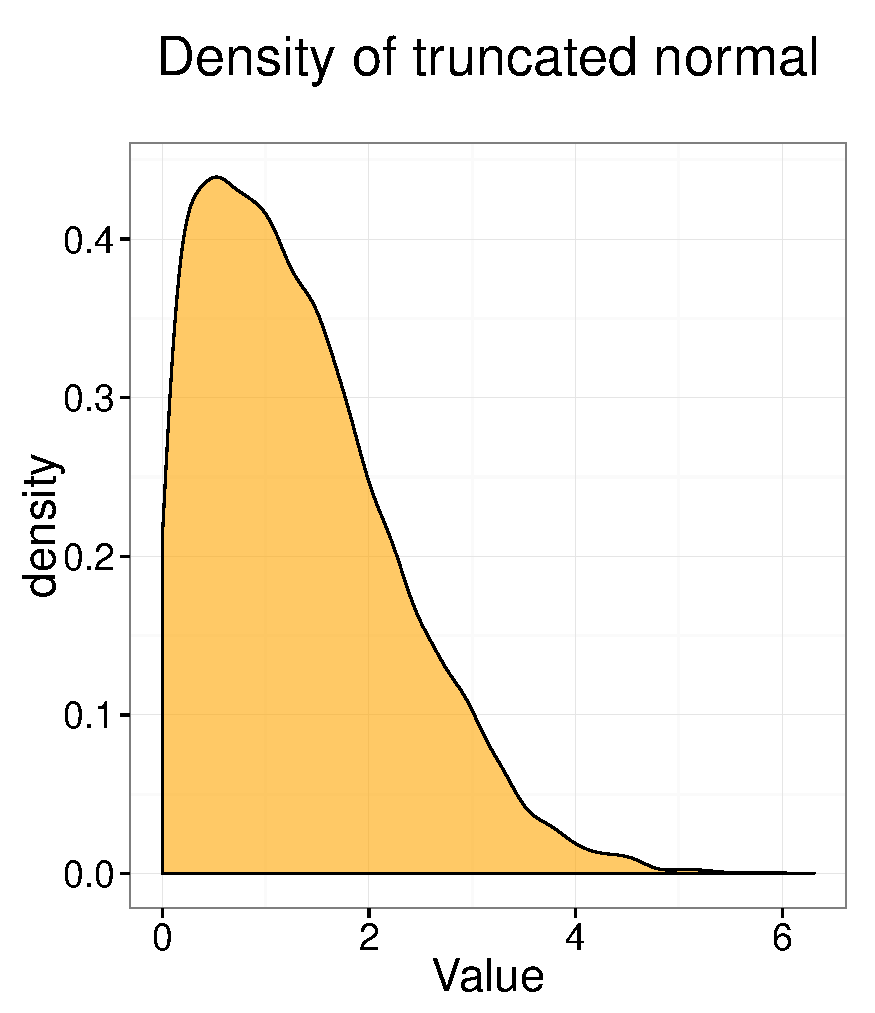
\includegraphics[width=300pt]{truncated_density.pdf}\\
  \label{density}
\end{figure}


\subsection*{Question 1 c) i}

To find the probability that the parameter $\theta$ lies between 0 and 1, all we need to do is find the proportion of draws from the distribution that are between 0 and 1.

\begin{verbatim}
  mean(draws>0 & draws<1)
\end{verbatim}

\noindent Which gives us $0.419$.

\subsection*{Question 1 c) ii)}

The 0.05 and 0.95 quantiles of the distribution are $[0.13, 3.12]$, which has a length of a little less than 3 (2.99).

\subsection*{Question 1 d)}

Given the distribution has a lot of mass at the truncation point, a 90 per cent credibility interval could probably contain that point. The $[0, 0.9]$ quantile interval, $[0, 2.65]$, is shorter, at only 2.65---a significant reduction.


\section*{Question 2: Method of Composition}

\subsection*{Question 2 a) i}

The program is a simple one. For each draw:

\begin{verbatim}
1. Draw a value of lambda from the inverted Gamma distribution
with shape

lambda = 1./gamrnd(nu/2, 2/nu, draws, 1)

2. Draw a value from the normal distribution with
the given mean and variance multiplied by lambda.

x = mu + (sqrt(sigma2*lambda)).*randn(draws, 1)
\end{verbatim}


\subsection*{Part 2 a) ii}

The program described above is implemented here:
\url{https://github.com/khakieconomics/homework/blob/master/Bayesian_econometrics/t_den_q2.m}

I have also sense-checked it in R, in particular by running a Kolmogorov-Smirnov test on the output of my sampler against a built-in sampler. The KS test is not rejected.

\url{https://github.com/khakieconomics/homework/blob/master/Bayesian_econometrics/Question_2.R}

\subsection*{Part 2 b)}

At 100k draws, the mean of the distribution is 1.004, and variance is 3.327.


\section*{Question 3: Linear Regression Model}

\subsection*{Question 3 a)}

The predictive density plot for the new observation is given. A simulated 90 per cent prediction interval for the sale of the new house is $[40602, 100354]$, both in dollars. The analytical interval is $[40273, 100663]$, though that calculation is made from a table whose greatest degrees of freedom is 200.

\begin{figure}
  \centering
  % Requires \usepackage{graphicx}
  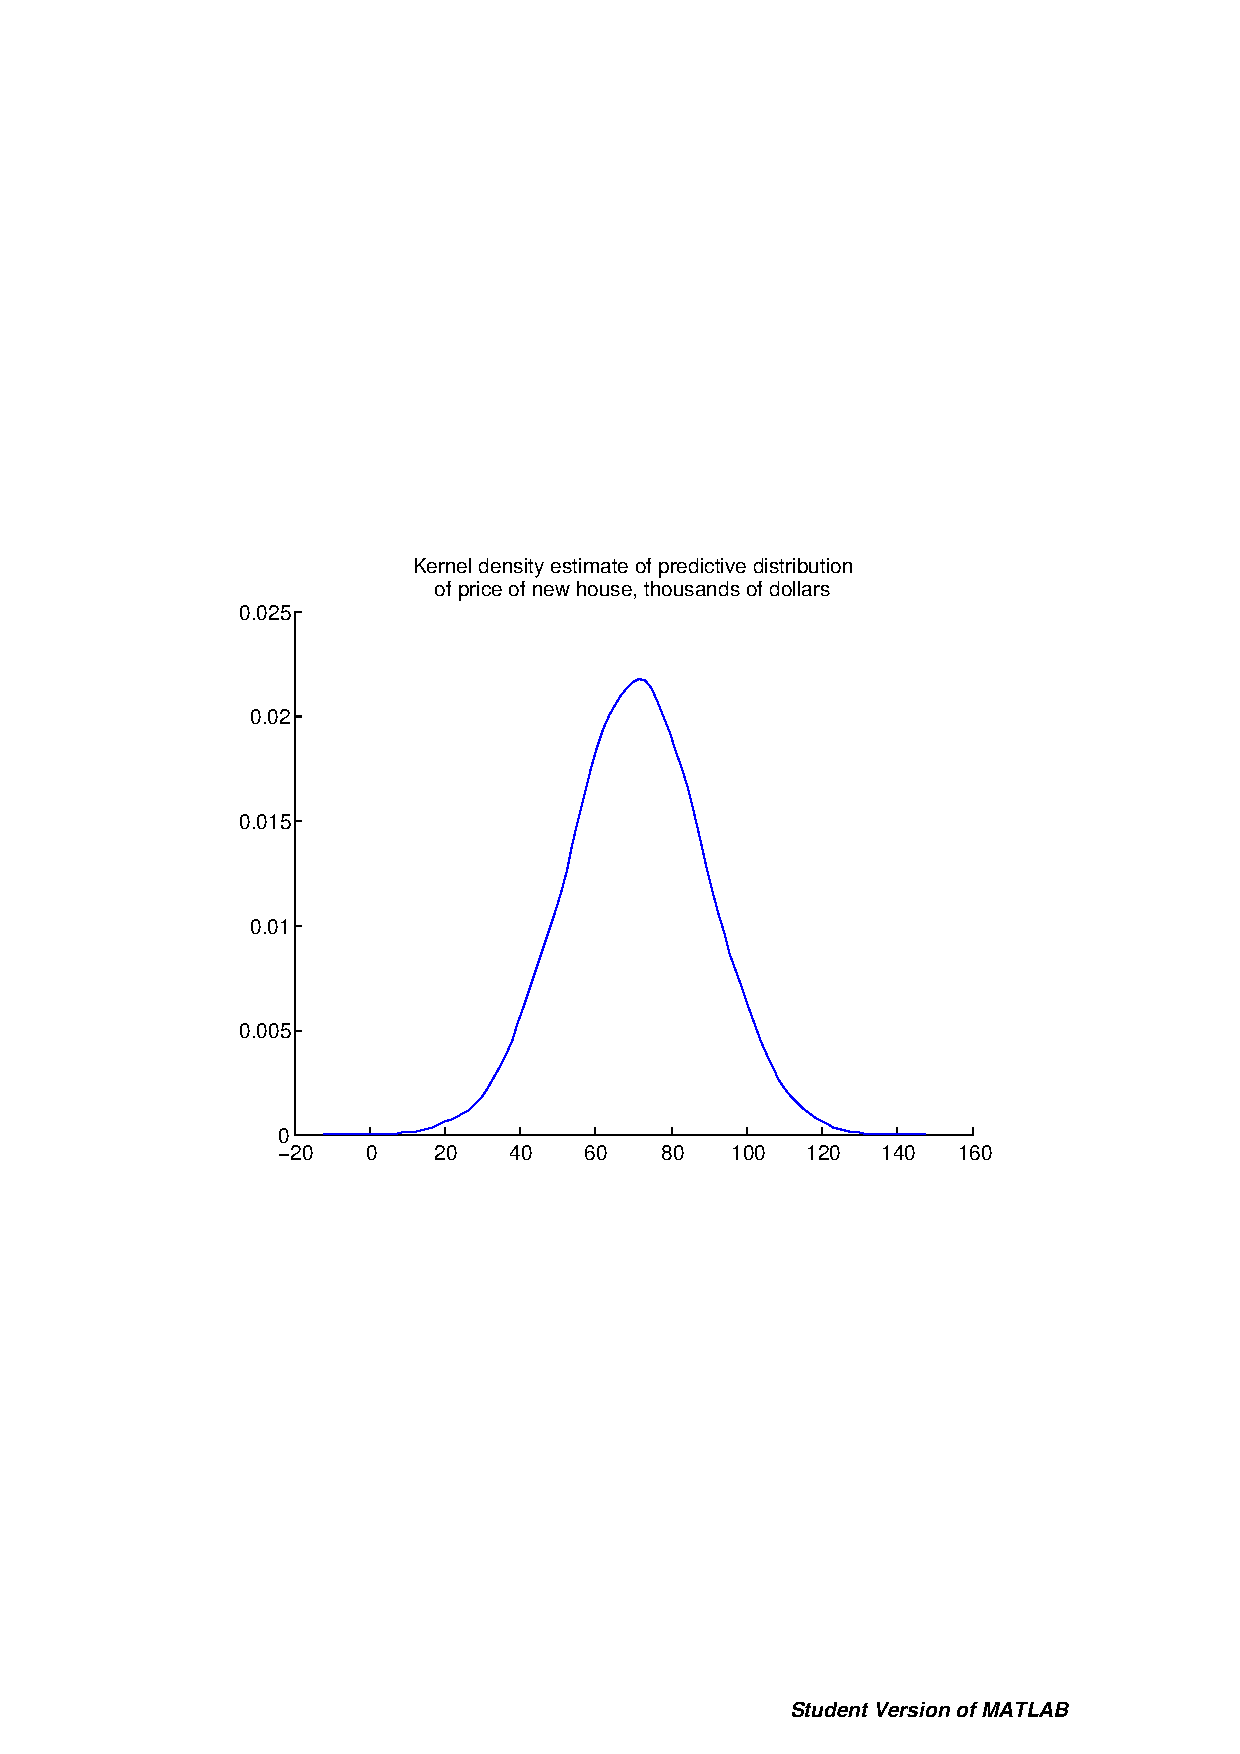
\includegraphics[width=300pt]{predictive_density.pdf}\\
  \label{preddensity}
\end{figure}

\subsection*{Question 3 b)}

Once all priors for $\beta$ are set to 0 (keeping variance priors unchanged), the 90 per cent HPDI becomes:\bigskip


\begin{centering}
  \begin{tabular}{|l|l|l|}
  \hline
  Variable & Lower 90 & Upper 90\\
  \hline
  % after \\: \hline or \cline{col1-col2} \cline{col3-col4} ...
  Intercept & -9497.05 & 2131.35 \\
  Lot size & 4.83 & 6.04 \\
  Number of bedrooms & 841.13 & 4774.29 \\
  Number of bathrooms & 14080.06 & 19706.31 \\
  Number of storeys & 6004.95 & 9289.14 \\
  $\sigma$ & 17286.43 & 19088.72 \\
  \hline
\end{tabular}

\end{centering}

\bigskip
Note that the $sigma$ HPDI is given as the standard error of the regression, not the variance. I find it easier to understand in this form.

\subsection*{Question 3 c}

The restricted model that takes house prices only as a function of the number of bedrooms and bathrooms results in the following estimates:

becomes:\bigskip


\begin{centering}
  \begin{tabular}{|l|l|l|l|}
  \hline
  Variable & Point estimate & Lower 90 & Upper 90 \\
  \hline
  % after \\: \hline or \cline{col1-col2} \cline{col3-col4} ...
  Intercept & 16677.3 & 10029.45 & 23325.14 \\
  Number of bedrooms & 7250.8 & 4995.57 & 9506.07 \\
  Number of bathrooms & 23280 & 19939.6 & 26620.42 \\
  $\sigma$ & 22250.01 & 21203.78 & 23414.48 \\
  \hline
\end{tabular}

\end{centering}

\bigskip

Note that comparing this model to the unrestricted model described above is essentially a joint test of whether lot size \emph{and} number of stories have no effect on the sale price of a house. In the Koop handout, restrictions on both of these variables had posterior odds ratios of practically zero, and so we'd expect the result to be heavily in favour of the unrestricted model.

Using a modified version of the Koop program, I worked out the posterior odds ratio for the restricted model relative to the unrestricted model. This is a tiny $7.16e-47$, suggesting that the restricted model does a poor job in comparison to the restricted model.

\section*{Question 4: Coins example}

The likelihood of a coin-toss where $h$ is the number of successes over $n$ flips with the probability of success being $\pi$ is given by the binomial distribution

\[
f(y|\pi) = {n \choose h} \pi^{h} (1-\pi)^{n-h}
\]

And the prior distribution is given by the [0,1] uniform distribution. As the Beta(1,1) distribution is uniform, and is also a conjugate prior to the binomial distribution, we use that. For the moment, we leave the prior distribution parameterised with $\alpha$ and $\beta$.

\[
p(\pi) = \frac{\Gamma(\alpha + \beta)}{\Gamma(\alpha)\Gamma(\beta)} \pi^{\alpha-1} (1-\alpha)^{\beta-1}
\]

The posterior is then given by Bayes rule:

\[
p(\pi|h) = \frac{{n \choose h} \pi^{h} (1-\pi)^{n-h}\times \frac{\Gamma(\alpha + \beta)}{\Gamma(\alpha)\Gamma(\beta)} \pi^{\alpha-1} (1-\alpha)^{\beta-1}}{\int_{0}^{1}{n \choose h} \pi^{h} (1-\pi)^{n-h}\times \frac{\Gamma(\alpha + \beta)}{\Gamma(\alpha)\Gamma(\beta)} \pi^{\alpha-1} (1-\alpha)^{\beta-1} d\pi}
\]

Which simplifies considerably

\[
p(\pi|h) = \frac{ \pi^{h + \alpha - 1} (1-\pi)^{n-h + \beta - 1}}{\int_{0}^{1}\pi^{h + \alpha - 1} (1-\pi)^{n-h + \beta - 1} d \pi}
\]

This is recognisable as the pdf of a beta distribution:

\[
p(\pi|h) = \frac{1}{Beta(h + \alpha, n - h + \beta)} \pi^{h + \alpha-1} (1-\pi)^{n-h + \beta-1}
\]

Where both $\alpha$ and $\beta$ are equal to $1$ under the uniform prior.

\subsection*{Question 4 ii}

As described above, the uniform distribution on the interval [0,1] can be expressed as a Beta(1,1) distribution. We like this, because it's a conjugate prior to the Binomial distribution, and possible to solve by hand.

The Beta(1,1) distribution is an example of a proper prior, in that it is integrable, and over the range [0,1] the integral evaluates at 1. Improper priors do not have this characteristic. While the Beta(1,1) prior here is proper, it is not particularly informative, as it places equal weight on all possible values of $\pi$.

\subsection*{Question 4 iii}

Using the parameterisation above, we can quite easily incorporate new prior information. This can be done by setting $\alpha=s_1$ and $\beta=s - s_1$.

\[
p(\pi|h) = \frac{1}{Beta(h + s_{1}, n - h + s - s_{1})} \pi^{h + s_{1}-1} (1-\pi)^{n-h + s - s_{1}-1}
\]


\section*{Question 5: Completing the squares}

\subsection*{Question 5 i}

For a model of the form $y = \mu + \epsilon$ with $\epsilon \sim \mathcal{N}(0, 1)$ for $n$ observations, we can express the likelihood function, in matrix form, as

\[
f(y|\mu) = \left(\frac{1}{2\pi}\right)^{\frac{n}{2}} \times \exp\left\{\frac{-1}{2}(y - \mu)'(y - \mu)\right\}
\]

Which simplifies as
\[
f(y|\mu) \propto \exp\left\{\frac{-1}{2}\sum_{1}^{n}(y_{i}-\mu)\right\}
\]

Using a prior $p(\mu) = \mathcal{N}(b_{0}, B_{0})$, which I express in proportional form, the posterior becomes

\[
p(\mu|y) \propto \exp\left\{\frac{-1}{2}\sum_{1}^{n}(y_{i}-\mu)^{2}\right\} \times \exp\left\{\frac{-1}{2B_{0}}(\mu-b_{0})^{2}\right\}
\]

\subsection*{Question 5 ii}

To use the complete the squares method, we first merge the exponents, take the squares of the terms in parentheses, and expand the brackets.

\[
p(\mu|y) \propto \exp\left\{\frac{1}{2} \sum_{-1}^{n} \left(y_{i}^{2} + \mu^{2} - 2y_{i}\mu \right) - \frac{1}{2B_{0}}\left(\mu^{2} + b_{0}^{2} - 2\mu b_{0}\right) \right\}
\]

\[
= \exp\left\{\frac{-1}{2} \sum_{1}^{n} y_{i}^{2} - \frac{1}{2}n\mu^{2} +\mu\sum_{i}^{n}y_{i} - \frac{\mu^{2}}{2B_{0}} - \frac{b_{0}^{2}}{2B_{0}} + \frac{\mu b_{0}}{B_{0}} \right\}
\]

Now we group the terms into a quadratic equation in $\mu$

\[
=\exp\left\{\frac{-\mu^{2}}{2}\left(n + \frac{1}{B_{0}}\right) + \mu\left(\sum_{1}^{n}y_{i} + \frac{b_{0}}{B_{0}}\right) - \frac{1}{2}\left(\sum_{1}^{n}y_{i} + \frac{b_{0}^{2}}{B_{0}}\right)\right\}
\]


What we really want are the moments of the following:
\[
\exp\left\{\frac{1}{2\sigma_{new}^{2}}\left(\mu-\mu_{new}\right)^{2}\right\}
\]

\[
=\exp \left\{\frac{1}{2\sigma_{new}^{2}} \left(\mu^{2}+\mu_{new}^{2} - 2 \mu \mu_{new}\right)\right\}
\]

From this expression, we match the coefficients of $\mu^{2}$

\[
\frac{-\mu^{2}}{2\sigma^{2}_{new}} = \frac{-\mu^{2}}{2} \left(n + \frac{1}{B_{0}}\right)
\]
\[
\rightarrow \sigma^{2}_{new} = \frac{1}{n + \frac{1}{B_{0}}}
\]

and of $\mu$

\[
\frac{-2\mu\mu_{new}}{2\sigma_{new}^{2}} = \mu\left(\sum y_{i} + \frac{b_{0}}{B_{0}}\right)
\]
\[
\rightarrow\mu_{new} = sigma_{new}^{2}\left(\sum y_{i} + \frac{b_{0}}{B_{0}}\right)
\]

And there we have the mean and variance of the posterior distribution!

\section*{Question 6: The accept-reject algorithm}

\subsection*{Answer!}

If we accept draws from $g(y)$ with probability $r(y)/cg(y)$ where $kr(y)=f(y)$ then:
\[
h\left(y|u\leq\frac{r(y)}{cg(y)}\right) = \frac{P\left(u<\frac{r(y)}{cg(y)}|y\right)g(y)}{\int P\left(u<\frac{r(y)}{cg(y)}|y\right)g(y)dy}
\]

due to the fact that for a uniform distribution $p(x<t)=t$,
\[
  =\frac{\frac{r(y)}{cg(y)}g(y)}{\int \frac{r(y)}{cg(y)}g(y)dy}
\]

And by definition of $r(y)$

\[
  =\frac{\frac{f(y)}{Kcg(y)}g(y)}{\int \frac{f(y)}{Kcg(y)}g(y)dy} = f(y)
\]

\emph{Voila!}
\end{document}
